%% ----------------------------------------------------------------
%% Thesis.tex -- main
%% ---------------------------------------------------------------- 

\documentclass[a4paper, 10pt, oneside]{memoir}
%% Use the option citeauthor to be able to use citet. The default cite will still work.
\usepackage[citeauthor]{basilea}

% Customizing captions
\usepackage{caption}
\captionsetup{
    labelformat=simple,
    font=small,
    labelfont=bf,
    justification=centering
}

% Code snippet support
\usepackage{listings}
\usepackage{xcolor}
% Configure Python syntax highlighting
\lstset{
    language=Python,
    basicstyle=\ttfamily\small,
    keywordstyle=\color{blue},
    commentstyle=\color{green!60!black},
    stringstyle=\color{red},
    numbers=left,
    numberstyle=\tiny\color{gray},
    stepnumber=1,
    numbersep=5pt,
    backgroundcolor=\color{gray!10},
    frame=single,
    frameround=tttt,
    breaklines=true,
    breakatwhitespace=false,
    showstringspaces=false,
    tabsize=2,
    captionpos=b
}

% Pseudo-code support
\usepackage{algorithm}
\usepackage{algpseudocode}

%% ----------------------------------------------------------------

\title				{Optimizing Symbolic Execution Through Taint Analysis and Path Prioritization}
\thesistype			{Bachelor thesis}

\department 		{Department of Mathematics and Computer Science}
\faculty			{Natural Science Faculty of the University of Basel}
\research		    {Databases and Information Systems (DBIS) Group \\ \url{https://dbis.dmi.unibas.ch/}}

\examiner    		{Dr. Marco Vogt}
\supervisor  		{Prof. Dr. Christopher Scherb}

\authors     		{Ruben Hutter}
\email				{ruben.hutter@unibas.ch}
\immatriculnr		{2020-065-934}

\date				{02.07.2025}

% switch here for the german logo to logo-de
\ulogo				{Template/logo-en} 


%% ----------------------------------------------------------------
\begin{document}

% for english use \selectlanguage{english}, for german use \selectlanguage{ngerman}
\selectlanguage{english}

\thesisfront
\maketitle
\pagestyle{thesis}
%% ----------------------------------------------------------------
% !TEX root = ../Thesis.tex
\chapter{Acknowledgments}

I would like to express my sincere gratitude to Prof. Dr. Christopher Scherb for his supervision and guidance throughout this thesis. His expertise in program analysis and symbolic execution provided essential direction for this research.

I am grateful to Dr. Marco Vogt for his role as examiner and for facilitating the opportunity to pursue this research topic. His feedback and suggestions helped refine both the technical approach and the presentation of this thesis.

I would like to thank Ivan Giangreco for providing the LaTeX thesis template used for this document, which greatly facilitated its formatting and structure.

I also acknowledge my fellow student Nico Bachmann for developing the Schnauzer visualization library, which enhanced the presentation and analysis of the results.

I thank my family and friends for their encouragement and support during my studies, which made completing this thesis possible.

Finally, I acknowledge the developers of the angr binary analysis framework, whose comprehensive platform enabled the implementation of the techniques described herein.

%% ----------------------------------------------------------------
% !TEX root = ../Thesis.tex
\chapter{Abstract}

Symbolic execution is a powerful program analysis technique widely used for vulnerability discovery and test case generation. However, its practical application is often hampered by scalability issues, primarily due to the "path explosion problem" where the number of possible execution paths grows exponentially with program complexity. This thesis addresses this fundamental challenge by proposing an optimized approach to symbolic execution that integrates taint analysis and path prioritization.

The core contribution is a novel exploration strategy that moves away from uniform path exploration towards targeted analysis of security-critical program behaviors. The approach prioritizes execution paths originating from memory allocations and user input processing points, as these represent common sources of vulnerabilities. By leveraging dynamic taint analysis, the system identifies and tracks data flow from these critical sources, enabling the symbolic execution engine to focus computational resources on paths influenced by tainted data while deprioritizing paths with no dependency on external inputs.

% TODO: Benchmark to test if this is actually true
The implementation integrates this taint-guided exploration strategy with the angr symbolic execution framework, introducing a scoring mechanism that dynamically adjusts path prioritization based on taint propagation. The effectiveness of this optimization is evaluated through comparative analysis, examining runtime efficiency, path coverage quality, and vulnerability discovery capabilities. Results demonstrate that this approach can significantly reduce the search space while maintaining or improving the detection of security-relevant program behaviors, making symbolic execution more practical for large and complex software systems.

%% ----------------------------------------------------------------
\thesistoc
%% ----------------------------------------------------------------
%\thesisnomencl
%% ----------------------------------------------------------------
\thesismain
% !TEX root = ../Thesis.tex
\chapter{Introduction}

Symbolic execution has emerged as one of the most powerful techniques for automated program analysis, offering significant advantages over traditional testing methods for vulnerability discovery and test case generation. By representing program inputs as symbolic variables rather than concrete values, symbolic execution engines can systematically explore multiple execution paths within a single analysis run, potentially uncovering bugs that would be difficult to find through conventional testing approaches.

Despite its theoretical promise, symbolic execution faces a fundamental scalability challenge known as the ``path explosion problem.'' As program complexity increases, the number of possible execution paths grows exponentially, quickly overwhelming computational resources and rendering the analysis intractable for real-world software systems. This limitation has been a persistent barrier to the widespread adoption of symbolic execution in practical security analysis workflows.

Current symbolic execution engines typically employ uniform exploration strategies, treating all program paths with equal priority regardless of their potential security relevance. This approach wastes significant computational resources on code paths that are unlikely to contain vulnerabilities, while potentially missing critical security-sensitive execution flows. For instance, paths that process user-controlled input or handle memory allocations are statistically more likely to contain exploitable vulnerabilities than paths that perform simple arithmetic operations or access read-only data structures.

This thesis addresses the path explosion problem by proposing a novel approach that integrates taint analysis with symbolic execution to enable intelligent path prioritization. The core insight is that not all execution paths are equally important from a security perspective. By leveraging taint analysis to identify and track data flow from critical sources such as user inputs and memory allocation sites, we can guide the symbolic execution engine to focus its computational resources on paths most likely to exhibit security-relevant behaviors.

The proposed approach introduces a dynamic scoring mechanism that continuously evaluates the security relevance of execution states based on taint propagation patterns. States that process tainted data receive higher priority scores, while states operating exclusively on untainted data are deprioritized or pruned entirely. This selective exploration strategy aims to maintain the thoroughness of symbolic execution for security-critical code while dramatically reducing the analysis time by avoiding exhaustive exploration of irrelevant program regions.

The main contributions of this work are:

\textbf{Taint-Guided Path Prioritization:} A novel integration of dynamic taint analysis with symbolic execution that uses taint propagation patterns to intelligently prioritize exploration of security-relevant execution paths.

\textbf{Adaptive Scoring Algorithm:} A scoring mechanism that dynamically adjusts path priorities based on real-time taint analysis results, enabling the symbolic execution engine to focus computational resources on the most promising program regions.

\textbf{Practical Implementation:} A complete implementation of the proposed approach using the angr symbolic execution framework, demonstrating the feasibility and effectiveness of taint-guided exploration in a production-quality tool.

\textbf{Empirical Evaluation:} Comprehensive evaluation comparing the proposed approach against standard symbolic execution techniques, measuring improvements in analysis efficiency, vulnerability discovery rate, and overall scalability.

The effectiveness of this optimization is evaluated through extensive experimentation on representative programs, examining key metrics including runtime efficiency, path coverage quality, and vulnerability detection capabilities. Results demonstrate that the taint-guided approach can significantly reduce analysis time while maintaining or improving the detection of security-relevant program behaviors, making symbolic execution more practical for analyzing large and complex software systems.

The remainder of this thesis is organized as follows. Chapter 2 provides essential background on symbolic execution, taint analysis, and the angr framework that forms the foundation for this work. Chapter 3 presents the conceptual framework and theoretical algorithms underlying the taint-guided exploration strategy. Chapter 4 details the practical implementation, including integration with angr and the design of the scoring mechanism. Chapter 5 presents a comprehensive evaluation of the approach, comparing its performance against standard symbolic execution techniques. Chapter 6 discusses related work in symbolic execution optimization and path prioritization. Chapter 7 concludes with a summary of contributions and implications for future research. Chapter 8 explores potential extensions and future research directions, while Chapter 9 documents the use of AI-assisted technologies in the development of this thesis.

% !TEX root = ../Thesis.tex
\chapter{Background}

This chapter establishes the theoretical foundations necessary for understanding the taint-guided symbolic execution optimization presented in this thesis. We examine symbolic execution, taint analysis, control flow analysis, and the Angr framework.

\section{Symbolic Execution}

Symbolic execution is a program analysis technique that explores execution paths by using symbolic variables instead of concrete inputs. The program state consists of symbolic variables, path constraints, and a program counter. When execution encounters a conditional branch, the engine explores both branches by adding appropriate constraints to the path condition.

A fundamental challenge in symbolic execution is the path explosion problem. As program complexity increases, the number of possible execution paths grows exponentially, making exhaustive exploration computationally intractable. This scalability issue particularly affects real-world applications with complex control flow structures and deep function call hierarchies. Research has shown that symbolic execution tools designed to optimize statement coverage often fail to cover potentially vulnerable code due to complex system interactions and scalability issues of constraint solvers \cite{schwartz_all_2010}.

Traditional symbolic execution typically employs a forward approach, starting from the program's entry point and exploring paths toward potential targets. However, this method may struggle to reach deeply nested functions or specific program locations of interest. Backward symbolic execution, conversely, begins from target locations and works backwards to identify input conditions that can reach those targets. Compositional approaches combine both techniques by analyzing individual functions in isolation and then reasoning about their interactions.

The scalability challenges of symbolic execution have motivated numerous optimization approaches, including state merging, constraint optimization, and path prioritization strategies. These optimization techniques form the foundation for more targeted analysis approaches that focus computational resources on security-relevant program behaviors.

\section{Taint Analysis}

Taint analysis tracks the propagation of data derived from untrusted sources throughout program execution. Data originating from designated sources (such as user input functions like \texttt{fgets}, \texttt{gets}, \texttt{read}, or \texttt{scanf}) is marked as ``tainted.'' The analysis tracks how this tainted data flows through assignments, function calls, and other operations. When tainted data reaches a security-sensitive sink (such as buffer operations or system calls), the analysis flags a potential vulnerability.

The propagation rules define how taint spreads through different operations: assignments involving tainted values result in tainted variables, arithmetic operations with tainted operands typically produce tainted results, and function calls with tainted arguments may result in tainted return values depending on the function's semantics. Dynamic taint analysis performs tracking during program execution, providing precise information about actual data flows while considering specific calling contexts and program states, resulting in reduced false positives compared to static analysis approaches.

The combination of taint analysis and symbolic execution creates a powerful analysis framework. Symbolic execution can explore multiple program paths while taint analysis identifies which paths involve security-relevant data flows. Research has demonstrated effective integration through pipelined approaches that achieve significant performance improvements while maintaining precision \cite{ming_taintpipe_2015}. This integration enables targeted exploration of paths that process untrusted input, significantly improving the efficiency of vulnerability discovery \cite{newsome_dynamic_2005}.

\section{Control Flow Analysis}

Control flow analysis examines the possible execution paths through a program by constructing and analyzing control flow graphs (CFGs). A CFG represents program structure where nodes correspond to basic blocks of sequential instructions and edges represent possible control transfers between blocks. This representation enables systematic analysis of program behavior and reachability properties.

Static analysis constructs CFGs by examining program code without executing it, analyzing structure and control flow based solely on the source code or binary representation. This approach offers comprehensive coverage and efficiency, enabling examination of all statically determinable program paths without requiring specific input values. However, static analysis faces limitations including difficulty with indirect call resolution and potential false positives due to conservative approximations required for soundness.

Dynamic analysis executes the program and collects runtime information, providing precise information about actual program behavior and complete execution context. This approach eliminates many false positives inherent in static analysis and validates that control flow relationships are actually exercised under realistic conditions. However, dynamic analysis results depend heavily on input quality and coverage.

A Call Graph represents function call relationships within a program, where each node corresponds to a function and each directed edge represents a call relationship. Call graphs serve important purposes including program understanding, entry point identification, reachability analysis, and complexity assessment. Call graphs prove valuable for path prioritization strategies, enabling identification of functions reachable from tainted input sources and assessment of their relative importance in program execution flow.

Modern analysis tools often combine both static and dynamic approaches. Hybrid techniques leverage the efficiency of static analysis for initial program understanding while using dynamic analysis to resolve ambiguities and validate findings under realistic execution conditions.

\section{Angr Framework}

Angr is an open-source binary analysis platform providing comprehensive capabilities for static and dynamic program analysis \cite{shoshitaishvili_sok_2016}. The platform supports multiple architectures and provides a Python-based interface for research and education \cite{springer_teaching_2018}. Key components include the Project object representing the binary under analysis with access to contents, symbols, and analysis capabilities; the Knowledge Base storing information gathered during analysis including function definitions and control flow graphs; the Simulation Manager handling multiple program states during symbolic execution and managing state transitions; and the Solver Engine interfacing with constraint solvers to determine path feasibility and solve for concrete input values.

Angr supports both static (\texttt{CFGFast}) and dynamic (\texttt{CFGEmulated}) CFG construction. Static analysis provides efficiency but may miss indirect calls, while dynamic analysis offers completeness at higher computational cost \cite{angr_documentation}. The static approach analyzes the binary without execution, making it efficient for initial program understanding, while dynamic analysis executes the program with sample inputs to discover reachable code, providing more complete coverage of actual execution paths and better handling of indirect calls.

Angr represents program states with register values, memory contents, path constraints, and execution history. The framework provides APIs for state inspection and manipulation, along with fine-grained execution control through step functions and exploration techniques. The step function advances execution by single instructions, enabling precise control over exploration processes, while various exploration strategies guide path selection including depth-first search, breadth-first search, and custom heuristics. Configuration options control execution behavior, such as handling of unconstrained memory and registers, allowing researchers to customize analysis behavior for specific research requirements.

The framework's extensible architecture enables integration of custom analysis techniques, making it particularly suitable for implementing novel symbolic execution optimizations. Angr's support for both static and dynamic analysis capabilities provides the foundation necessary for implementing taint-guided exploration strategies that combine control flow analysis with symbolic execution.

Multiple symbolic execution frameworks have been developed to address the scalability challenges discussed earlier \cite{baldoni_survey_2018}. While angr focuses on binary analysis and provides a comprehensive platform for security research, other frameworks target different domains and approaches. KLEE \cite{cadar_klee_2008} remains one of the most prominent tools for C programs, focusing on automatic test generation and providing extensive coverage analysis capabilities. SAGE \cite{godefroid_automated_2008} extends symbolic execution to binary code analysis through whitebox fuzzing, particularly effective for vulnerability discovery in Windows applications. CBMC \cite{clarke_behavioral_2003} offers bounded model checking for C/C++ programs with formal verification capabilities. Java PathFinder \cite{visser_model_2003} provides symbolic execution for Java bytecode with emphasis on model checking applications. Each framework offers distinct advantages: KLEE excels in systematic path exploration for source code, SAGE in practical vulnerability discovery for binaries, CBMC in formal verification, and Java PathFinder in model checking for Java applications.

% !TEX root = ../Thesis.tex
\chapter{Related Work}\label{ch:related_work}

This chapter surveys existing research in symbolic execution optimization and taint analysis techniques, positioning TraceGuard within the broader landscape of security-focused program analysis. We examine three primary categories of approaches: optimization strategies for managing path explosion, integration techniques combining multiple analysis methods, and security-oriented targeting approaches.

\section{Optimization Approaches}

\subsection{State Space Reduction}

The fundamental challenge in symbolic execution remains the path explosion problem, where the number of execution paths grows exponentially with program complexity. \citet{kuznetsov_efficient_2012} introduced efficient state merging techniques to reduce symbolic execution states by combining states with similar path conditions. While effective for certain program structures, this approach lacks security-focused guidance, treating all execution paths equally regardless of their interaction with potentially malicious inputs.

\citet{avgerinos_enhancing_2014} proposed AEG (Automatic Exploit Generation), which prioritizes paths leading to exploitable conditions. However, AEG relies primarily on static analysis to identify potentially vulnerable locations, missing dynamic taint flow patterns that emerge only during execution.

Recent work by \citet{yao_empc_2025} introduces Empc, a path cover-based approach that leverages minimum path covers (MPCs) to reduce the exponential number of paths while maintaining code coverage. However, Empc focuses on maximizing code coverage efficiently, while TraceGuard specifically targets security-relevant execution paths through taint propagation analysis.

\subsection{Performance and Compositional Analysis}

\citet{poeplau_symbolic_2020} developed optimizations for constraint solving by caching frequently encountered constraints. While these optimizations improve execution speed, they do not address the fundamental issue of exploring irrelevant paths that have no security implications.

\citet{ognawala_macke_2016} introduced MACKE, a compositional approach that analyzes functions in isolation before combining results. This technique encounters difficulties when taint flows cross function boundaries, as compositional analysis may miss inter-procedural data dependencies crucial for security analysis.

\section{Integration Approaches}

Dynamic taint analysis and symbolic execution represent complementary approaches that, when combined effectively, can overcome individual limitations. \citet{schwartz_all_2010} provide a comprehensive comparison of dynamic taint analysis and forward symbolic execution, noting that taint analysis excels at tracking data flow patterns but lacks the path exploration capabilities of symbolic execution. Their work identifies the potential for hybrid approaches but does not present a concrete integration strategy.

\citet{ming_taintpipe_2015} developed TaintPipe, a pipelined approach to symbolic taint analysis that performs lightweight runtime logging followed by offline symbolic taint propagation. While TaintPipe demonstrates the feasibility of combining taint tracking with symbolic reasoning, it operates in a post-processing mode rather than providing real-time guidance to symbolic execution engines.

Recent hybrid fuzzing approaches combine fuzzing with selective symbolic execution but lack sophisticated taint-awareness in their path prioritization strategies. These tools typically trigger symbolic execution when fuzzing coverage stagnates, rather than using taint information to proactively guide exploration toward security-relevant program regions.

\section{Security-Focused Targeting and Research Gap}

Security-focused symbolic execution approaches attempt to prioritize execution paths that are more likely to contain vulnerabilities. Static vulnerability detection approaches rely on pattern matching and dataflow analysis to identify potentially dangerous code locations, but cannot capture the dynamic taint propagation patterns that characterize real security vulnerabilities. Binary analysis frameworks like Angr~\cite{shoshitaishvili_sok_2016} provide powerful symbolic execution capabilities but lack built-in security-focused exploration strategies.

The literature survey reveals critical limitations that TraceGuard addresses: (1) \textbf{Lack of Dynamic Taint-Guided Prioritization} - existing approaches focus on general path reduction rather than security-specific targeting; (2) \textbf{Reactive Integration Strategies} - current techniques use taint analysis in post-processing roles rather than as primary exploration drivers; (3) \textbf{Limited Security-Awareness} - optimizations treat all paths equally, failing to recognize higher vulnerability potential of taint-processing paths.

TraceGuard addresses these limitations through a novel real-time integration of dynamic taint analysis with symbolic execution, representing the first comprehensive framework for leveraging runtime taint information to intelligently prioritize security-relevant execution paths.

% !TEX root = ../Thesis.tex
\chapter{Taint-Guided Exploration}\label{ch:taint_guided_exploration}

Having established the theoretical foundations in Chapter~\ref{ch:background} and surveyed existing approaches in Chapter~\ref{ch:related_work}, this chapter presents the conceptual framework and algorithmic design of TraceGuard's taint-guided symbolic execution strategy. Rather than exploring all possible execution paths uniformly, TraceGuard prioritizes paths based on their interaction with potentially malicious user input, fundamentally addressing the path explosion problem through intelligent exploration guidance.

The core insight underlying this approach is that security vulnerabilities are significantly more likely to occur in code paths that process external, user-controlled data. By tracking taint flow from input sources and using this information to guide symbolic execution, TraceGuard focuses computational resources on security-relevant program regions while avoiding exhaustive exploration of paths that operate solely on trusted internal data.

\section{Core Approach}

TraceGuard operates as a specialized program built on the Angr framework that transforms symbolic execution from exhaustive path exploration into a security-focused analysis. The approach centers on four key mechanisms that work together to prioritize execution paths based on their interaction with potentially malicious user input.

\textbf{Hook-Based Taint Detection:} The system intercepts function calls during symbolic execution to identify when external data enters the program. Input functions like \texttt{fgets} and \texttt{scanf} are immediately flagged as taint sources, while other functions are monitored for tainted parameter usage.

\textbf{Symbolic Taint Tracking:} Tainted data is tracked through unique symbolic variable names and memory region mappings. When input functions create symbolic data, the variables receive distinctive ``\texttt{taint\_source\_}'' prefixes that persist throughout symbolic execution.

\textbf{Dynamic State Prioritization:} Each symbolic execution state receives a taint score based on its interaction with tainted data. States are classified into three priority levels that determine exploration order: high priority (score $\geq \tau_{high}$), medium priority ($\tau_{medium} \leq$ score $< \tau_{high}$), and normal priority (score $< \tau_{medium}$).

\textbf{Exploration Boundaries:} Multiple complementary techniques prevent path explosion: execution length limits, loop detection, and graduated depth penalties that naturally favor shorter paths to vulnerability-triggering conditions.

\vspace{1em}

Throughout the following algorithms, we use configurable parameters to maintain generality: $\alpha_{input}$ represents the score bonus for input function interactions, $\beta_{tainted}$ denotes the bonus for execution within tainted functions, $\gamma_{penalty}$ specifies the depth penalty multiplication factor, $\delta_{threshold}$ defines the depth threshold for penalty application, $\sigma_{min}$ sets the minimum exploration score, $\tau_{high}$ and $\tau_{medium}$ establish the priority classification thresholds, and $k$ determines the maximum number of active states. In our implementation, these parameters are set to $\alpha_{input} = 5.0$, $\beta_{tainted} = 3.0$, $\gamma_{penalty} = 0.95$, $\delta_{threshold} = 200$, $\sigma_{min} = 1.0$, $\tau_{high} = 6.0$, $\tau_{medium} = 2.0$, and $k = 15$.

\section{Taint Source Recognition}\label{sec:taint_source_recognition}

TraceGuard identifies taint sources by hooking functions during program analysis. This hook-based approach enables runtime detection of external data entry points without requiring complex static analysis.

\begin{algorithm}[H]
\caption{Function Hooking Strategy}\label{alg:function_hooking}
\begin{algorithmic}[1]
\Require Program binary $P$
\State $CFG \gets \textsc{BuildControlFlowGraph}(P)$
\State $InputFunctions \gets \{\text{fgets, scanf, read, gets}\}$
\ForAll{function $f$ in $CFG$}
    \If{$f.name \in InputFunctions$}
        \State $\textsc{InstallInputHook}(f)$
    \Else
        \State $\textsc{InstallGenericHook}(f)$
    \EndIf
\EndFor
\end{algorithmic}
\end{algorithm}

The system uses two types of hooks: input function hooks that immediately mark data as tainted, and generic hooks that check whether function parameters contain tainted data. This dual approach ensures both taint introduction and propagation are monitored throughout execution.

Input functions receive special treatment because they represent the primary vectors for external data entry. When these functions are called, the system automatically creates tainted symbolic data and registers the associated memory regions as containing potentially malicious content.

\section{Dynamic Taint Tracking}\label{sec:dynamic_taint_tracking}

TraceGuard tracks taint propagation through two complementary mechanisms: symbolic variable naming and memory region mapping. This approach ensures taint information persists across function calls and memory operations.

\begin{algorithm}[H]
\caption{Taint Introduction at Input Functions}
\begin{algorithmic}[1]
\Require Function call to input function $f$, State $s$
\State $data \gets \textsc{CreateSymbolicData}(\text{taint\_source\_} + f.name)$
\State $s.globals[\text{taint\_score}] \gets s.globals[\text{taint\_score}] + \alpha_{input}$
\State $s.globals[\text{tainted\_functions}].add(f.name)$
\If{$f$ involves memory allocation}
    \State $buffer\_addr \gets \textsc{GetBufferAddress}(s)$
    \State $buffer\_size \gets \textsc{GetBufferSize}(s)$
    \State $s.globals[\text{tainted\_regions}].add((buffer\_addr, buffer\_size))$
\EndIf
\State \Return $data$
\end{algorithmic}
\end{algorithm}

Symbolic variable naming creates a persistent taint identifier that follows data through symbolic operations. Memory region tracking maintains a mapping of tainted buffer addresses and sizes, enabling taint detection when pointers reference previously tainted memory locations.

\begin{algorithm}[H]
\caption{Taint Status Check}
\begin{algorithmic}[1]
\Require State $s$, Variable or address $target$
\If{$target$ is symbolic variable}
    \State \Return $\text{taint\_source\_} \in target.name$
\ElsIf{$target$ is memory address}
    \ForAll{$(addr, size)$ in $s.globals[\text{tainted\_regions}]$}
        \If{$addr \leq target < addr + size$}
            \State \Return $\textsc{True}$
        \EndIf
    \EndFor
\EndIf
\State \Return $\textsc{False}$
\end{algorithmic}
\end{algorithm}

Additionally, memory region tracking maintains a mapping of tainted buffer addresses and sizes, enabling taint detection when pointers reference previously tainted memory locations.

\section{Path Prioritization}\label{sec:path_prioritization}

TraceGuard implements a three-tier prioritization system that classifies symbolic execution states based on their calculated taint scores. This classification determines exploration order to focus computational resources on security-relevant paths.

\begin{algorithm}[H]
\caption{State Classification and Prioritization}
\begin{algorithmic}[1]
\Require Active states $\mathcal{S}$, Thresholds $\tau_{high}$, $\tau_{medium}$
\State $scored\_states \gets []$
\ForAll{state $s \in \mathcal{S}$}
    \State $score \gets \textsc{CalculateTaintScore}(s)$
    \State $scored\_states.append((score, s))$
\EndFor
\State $P_{high} \gets \{s : score \geq \tau_{high}\}$
\State $P_{medium} \gets \{s : \tau_{medium} \leq score < \tau_{high}\}$ 
\State $P_{normal} \gets \{s : score < \tau_{medium}\}$
\State exploration\_queue $\gets P_{high} + P_{medium} + P_{normal}$
\State \Return first $k$ states from exploration\_queue
\end{algorithmic}
\end{algorithm}

The score calculation combines multiple factors to assess security relevance. Base scores come from taint interactions tracked by function hooks, with additional bonuses for execution within previously identified tainted functions and penalty reductions for excessive execution depth.

\begin{algorithm}[H]
\caption{Taint Score Calculation}
\begin{algorithmic}[1]
\Require State $s$
\State $score \gets \max(s.globals[\text{taint\_score}], \sigma_{min})$
\If{current function $\in$ tainted functions}
    \State $score \gets score + \beta_{tainted}$
\EndIf
\If{execution depth $> \delta_{threshold}$}
    \State $score \gets score \times \gamma_{penalty}$
\EndIf
\State \Return $score$
\end{algorithmic}
\end{algorithm}

High-priority states typically represent paths directly processing user input or executing within security-critical functions. Medium-priority states show moderate taint relevance, while normal-priority states primarily handle untainted data. The system limits active states to prevent path explosion while maintaining adequate exploration coverage.

\subsection{Adaptive State Pool Management}

A critical component of TraceGuard's practical viability lies in its adaptive state pool management strategy, which prevents path explosion while maintaining exploration effectiveness. The system employs a bounded exploration approach that dynamically adjusts the active state pool based on both computational constraints and taint score distributions.

\textbf{Bounded Exploration Principle:} Rather than allowing unlimited state proliferation, TraceGuard maintains a fixed upper bound $k$ on concurrent active states. This constraint transforms the potentially infinite symbolic execution search space into a manageable, resource-bounded exploration process. The bound $k$ represents a balance between exploration thoroughness and computational tractability, typically set to a small constant based on empirical analysis of memory usage and solver performance.

\textbf{Dynamic State Replacement:} When the exploration encounters new states that would exceed the bound $k$, the system employs a replacement strategy based on taint scores. New states are only admitted to the active pool if their taint scores exceed those of current low-priority states. This ensures that computational resources remain focused on the most security-relevant execution paths, even as the program exploration discovers new branches.

\textbf{Priority-Based Pruning:} The state pruning mechanism operates according to the established three-tier priority system. When resource limits are reached, normal-priority states are pruned first, followed by medium-priority states if necessary. High-priority states are preserved except in extreme cases where all active states achieve high-priority classification, at which point fine-grained score comparisons determine pruning order.

This adaptive approach ensures that TraceGuard maintains bounded computational requirements while maximizing the security relevance of explored paths, addressing both the theoretical challenge of path explosion and the practical constraints of finite computational resources.

\section{Exploration Depth Control and Vulnerability Probability}\label{sec:exploration_depth_control}

TraceGuard prevents path explosion through multiple complementary techniques that limit exploration depth while maintaining sufficient coverage for vulnerability discovery. A fundamental principle underlying this approach is the inverse relationship between execution depth and vulnerability probability.

The preference for shorter paths in vulnerability discovery is grounded in both theoretical security principles and empirical evidence from vulnerability research~\cite{schwartz_all_2010}. Security vulnerabilities typically manifest near the boundary between external input and internal program logic, where insufficient validation or sanitization allows malicious data to corrupt program state. As execution depth increases beyond these initial input processing stages, several factors reduce vulnerability probability: (1) input data has undergone additional validation and transformation steps, (2) the program state becomes more complex and harder for attackers to predict and control, and (3) deeper code paths typically receive more thorough testing during development.

Research on real-world vulnerability databases demonstrates that critical security flaws such as buffer overflows and injection attacks are statistically more likely to occur in shallow call stacks near input sources than in deeply nested program logic. This observation aligns with attack surface theory, which suggests that the most accessible vulnerabilities are those that can be triggered with minimal program state setup, making them both more discoverable by automated tools and more attractive to attackers.

\begin{algorithm}[H]
\caption{Progressive Depth Penalties}
\begin{algorithmic}[1]
\Require State $s$ with execution depth $d$
\If{$d > \delta_{high}$}
    \State $s.score \gets s.score \times \gamma_{high}$
\ElsIf{$d > \delta_{medium}$}
    \State $s.score \gets s.score \times \gamma_{medium}$
\EndIf
\end{algorithmic}
\end{algorithm}

The depth penalty system gradually reduces state scores as execution depth increases, naturally prioritizing shorter paths that are more likely to trigger vulnerabilities quickly. This graduated approach avoids abrupt path termination while steering exploration toward more promising regions of the program space. The system employs configurable depth thresholds ($\delta_{high}$, $\delta_{medium}$) and penalty factors ($\gamma_{high}$, $\gamma_{medium}$) to balance thorough exploration with computational efficiency.

Beyond depth penalties, TraceGuard coordinates multiple exploration control mechanisms to manage path explosion effectively. These include execution length limitations to prevent infinite loops, cycle detection to avoid repetitive exploration patterns, and adaptive state management that maintains an optimal number of active states based on available computational resources.

% !TEX root = ../Thesis.tex
\chapter{Implementation}

This chapter presents the practical realization of the taint-guided symbolic execution approach described in Chapter~\ref{ch:taint_guided_exploration}. The implementation, named TraceGuard, is built using Python and integrates with the Angr binary analysis framework to provide taint-aware symbolic execution capabilities. Following the architectural principles established in the theoretical approach, TraceGuard demonstrates how dynamic taint analysis can be effectively integrated with symbolic execution to achieve security-focused path prioritization.

The chapter is structured to first present the overall system architecture and design principles (Section~\ref{sec:system_architecture}), followed by detailed descriptions of the core implementation components (Sections~\ref{sec:angr_integration} through~\ref{sec:configuration_and_usage}). Finally, Section~\ref{sec:implementation_validation} discusses practical usage considerations and deployment strategies.

\section{System Architecture}\label{sec:system_architecture}

TraceGuard operates as a Python-based tool that extends Angr's symbolic execution capabilities with taint-guided exploration techniques. The system architecture follows a modular design centered around the \texttt{TaintAnalyzer} class, which coordinates all analysis components. The tool consists of five primary subsystems that work together to provide comprehensive taint-guided analysis.

\textbf{Project Management Subsystem:} The \texttt{TaintAnalyzer} class handles Angr project initialization, binary loading, and configuration management. This subsystem manages the overall analysis workflow and coordinates between different components.

\textbf{Control Flow Analysis Subsystem:} Builds and analyzes the program's control flow graph (CFG) to identify function boundaries and call relationships. This subsystem provides the foundation for function hooking and taint propagation analysis.

\textbf{Function Hooking Subsystem:} Implements comprehensive function interception capabilities using Angr's hooking mechanism. This subsystem distinguishes between input functions that introduce taint and generic functions that propagate taint.

\textbf{Taint Tracking Subsystem:} Manages taint detection, propagation, and state scoring throughout symbolic execution. This subsystem implements the core taint analysis logic that identifies when data from input sources flows through the program.

\textbf{Exploration Control Subsystem:} Integrates the custom \texttt{TaintGuidedExploration} technique with Angr's simulation manager to prioritize states based on taint information. This subsystem ensures that security-relevant execution paths receive computational priority.

\subsection{Core Design Principles}

The implementation follows several key design principles that ensure both effectiveness and maintainability. \textbf{Modular Architecture} ensures that each component has well-defined responsibilities and interfaces, enabling independent modification and testing of individual subsystems.

\textbf{Angr Framework Integration} maintains full compatibility with existing Angr workflows while adding specialized taint-guided capabilities. The implementation leverages Angr's established patterns for project management, symbolic execution, and exploration techniques.

\textbf{Configurable Analysis Parameters} allows users to customize taint sources, exploration limits, and logging levels based on their specific analysis requirements. This flexibility enables adaptation to different types of security analysis scenarios.

\textbf{Comprehensive Function Coverage} ensures that all user-defined functions are monitored for taint interaction, while essential system functions receive special handling to maintain analysis stability.

\section{Angr Integration Layer}\label{sec:angr_integration}

\subsection{Project Initialization and Setup}

The core implementation begins with the \texttt{TaintAnalyzer} class constructor, which handles all aspects of Angr project setup and configuration. The initialization process follows a structured sequence that ensures reliable analysis foundation.

Binary loading utilizes Angr's standard project creation mechanisms with automatic architecture detection and symbol resolution. The system identifies the main function through symbol table analysis, falling back to the program entry point when necessary.

Control flow graph construction employs Angr's CFGFast analysis to build a comprehensive function map that includes both user-defined and library functions. This CFG serves as the foundation for subsequent function hooking and taint propagation analysis.

Architecture-specific configuration automatically detects the target architecture (AMD64 or x86) and configures appropriate argument passing conventions. This ensures accurate taint tracking across function boundaries regardless of the target platform.

\subsection{Custom Exploration Technique}

The \texttt{TaintGuidedExploration} class extends Angr's \texttt{ExplorationTechnique} framework to provide taint-aware state prioritization. This class implements the state classification and prioritization algorithms described in Chapter~\ref{ch:taint_guided_exploration}, serving as the primary interface between taint analysis results and symbolic execution control decisions.

The exploration technique maintains comprehensive metrics on tainted versus untainted state exploration, providing insights into the effectiveness of the prioritization strategy. When Angr's simulation manager selects states for exploration, the technique reorders the active state list based on computed taint scores.

State classification operates through a scoring system that evaluates each state's interaction with tainted data. States that process tainted data receive higher priority scores, while states operating solely on untainted data receive lower scores. This classification ensures that security-relevant execution paths are explored before less critical alternatives.

The technique integrates with TraceGuard's taint tracking infrastructure by accessing project-level taint information, including tracked function calls and tainted memory regions. This integration enables dynamic prioritization based on real-time taint analysis results.

\subsection{State Scoring Implementation}

State scoring in TraceGuard operates through a multi-factor algorithm that evaluates several dimensions of taint interaction. The scoring system maintains individual scores for each active symbolic execution state, updating these scores as execution progresses.

Function call taint scoring assigns higher scores to states that call functions with tainted parameters, implementing the prioritization logic described in Algorithm~\ref{alg:function_hooking}. Input function calls receive the highest score bonus, followed by calls to functions that process tainted data.

Execution context scoring considers the current function context and its relationship to tainted data flow. States executing within functions known to process tainted data receive sustained score bonuses, ensuring continued prioritization throughout tainted execution paths.

Score decay mechanisms prevent indefinite prioritization of states that may have processed tainted data in the past but are no longer actively interacting with it. This decay ensures that exploration remains focused on currently relevant taint interactions.

\section{Taint Tracking Implementation}\label{sec:taint_tracking_implementation}

\subsection{Function Hooking Strategy}

TraceGuard implements comprehensive function hooking through a two-tier strategy that distinguishes between input functions and generic functions. The hooking system intercepts all function calls during symbolic execution to monitor taint introduction and propagation.

Input function hooks target specific functions known to introduce external data into the program, including \texttt{fgets}, \texttt{scanf}, \texttt{read}, and \texttt{gets}. These hooks automatically create tainted symbolic data with distinctive variable names that enable tracking throughout program execution.

Generic function hooks monitor all other user-defined functions to detect when tainted data is passed as parameters. These hooks examine function arguments using architecture-specific calling conventions to identify taint propagation across function boundaries.

Hook implementation utilizes Angr's SimProcedure mechanism to intercept function calls without disrupting normal program execution flow. The hooks maintain detailed statistics on function execution patterns and taint interaction frequency.

\subsection{Taint Source Detection}

Taint source detection operates through runtime analysis of function parameters and return values. The system identifies taint sources by monitoring specific input functions and automatically marking their outputs as tainted.

Symbolic variable naming provides the primary mechanism for taint identification. Input functions create symbolic variables with the prefix \texttt{taint\_source\_}, enabling persistent identification throughout symbolic execution. This naming convention ensures that tainted data remains identifiable even after complex transformations.

Memory region tracking complements symbolic variable naming by maintaining a registry of memory addresses that contain tainted data. This dual approach ensures comprehensive taint detection for both register-based and memory-based data flow.

Parameter taint analysis examines function call arguments to determine which parameters carry tainted data. The system uses architecture-specific register mappings to correctly identify tainted parameters across different calling conventions.

\subsection{Taint Propagation Engine}

The taint propagation engine tracks how tainted data flows through the program using both symbolic analysis and memory tracking. This engine ensures that taint information remains accurate as data moves between variables, memory locations, and function boundaries.

Symbolic taint propagation leverages Angr's symbolic execution engine to automatically track tainted variables through arithmetic operations, assignments, and control flow decisions. The system maintains taint information through symbolic variable dependencies and transformations.

Memory-based taint tracking monitors when tainted data is stored to or loaded from memory locations. The system maintains a registry of tainted memory regions that is updated whenever tainted data is written to memory or when memory contents are modified.

Inter-function taint flow ensures that taint information propagates correctly across function call boundaries. The system tracks both parameter passing and return value propagation to maintain taint accuracy throughout complex function call hierarchies.

\subsection{Architecture-Specific Implementation}

TraceGuard supports both AMD64 and x86 architectures through configurable parameter passing conventions. The system automatically detects the target architecture and configures appropriate register mappings for argument analysis.

AMD64 support utilizes the standard System V calling convention with arguments passed in \texttt{rdi}, \texttt{rsi}, \texttt{rdx}, \texttt{rcx}, \texttt{r8}, and \texttt{r9} registers. The system correctly handles both register and stack-based parameter passing for functions with many arguments.

x86 support implements the standard calling convention with stack-based parameter passing. The system adjusts memory offset calculations to correctly identify function parameters on the x86 stack layout.

Architecture detection occurs automatically during project initialization, ensuring that the correct calling convention is applied without user intervention. This automatic configuration enables cross-platform analysis without manual parameter adjustment.

\section{Configuration and Usage}\label{sec:configuration_and_usage}

\subsection{Command-Line Interface}

TraceGuard provides a comprehensive command-line interface that enables flexible configuration of analysis parameters. The interface supports both basic usage for quick analysis and advanced options for detailed customization.

Basic usage requires only the target binary path: \texttt{python taint\_se.py <binary\_path>}. This command performs a complete taint-guided analysis using default parameters suitable for most security analysis scenarios.

Logging configuration options include \texttt{--verbose} for detailed execution information and \texttt{--debug} for comprehensive debugging output. These options enable users to monitor analysis progress and troubleshoot potential issues.

Advanced options include \texttt{--meta-file} for specifying custom function parameter information and visualization flags for generating graphical representations of taint flow patterns.

\subsection{Integration Workflow}

TraceGuard integrates into existing binary analysis workflows through a straightforward execution model that requires minimal setup. The tool automatically handles Angr project configuration and symbolic execution setup.

Analysis execution proceeds through several distinct phases: binary loading and CFG construction, function identification and hooking, symbolic execution with taint tracking, and result reporting. Each phase provides progress feedback and error handling to ensure robust analysis completion.

Result interpretation focuses on identifying functions that process tainted data and execution paths that demonstrate taint flow from input sources to critical program locations. The tool provides detailed logs showing which functions were executed versus skipped based on taint status.

Visualization capabilities enable graphical representation of call graphs with taint information, highlighting security-relevant execution paths and function relationships. This visualization assists analysts in understanding complex taint flow patterns.

\subsection{Performance Considerations}

The implementation incorporates several performance optimizations to manage the computational overhead of comprehensive taint tracking. These optimizations address the additional analysis requirements while maintaining acceptable execution performance.

Function hooking optimization minimizes overhead by using efficient parameter checking mechanisms that avoid unnecessary symbolic computation. The system only performs detailed taint analysis when function parameters potentially contain tainted data.

Exploration technique integration ensures that taint-guided prioritization enhances rather than impedes symbolic execution performance. The prioritization overhead is minimal compared to the benefits of focusing analysis on security-relevant paths.

Memory management optimizations minimize the storage requirements for taint tracking information. The system uses efficient data structures and garbage collection strategies to prevent memory consumption from growing unboundedly during long-running analyses.

\section{Implementation Validation}\label{sec:implementation_validation}

The TraceGuard implementation has been validated through comprehensive testing using both synthetic test programs and real-world binary samples. The validation process confirms that the implementation correctly realizes the theoretical algorithms described in Chapter~\ref{ch:taint_guided_exploration} while maintaining acceptable performance characteristics.

Functional validation verifies that taint tracking operates correctly across diverse program constructs, including complex control flow patterns, multiple input sources, and inter-procedural data flow. The testing suite includes programs specifically designed to exercise edge cases in taint propagation logic.

Architecture validation confirms correct operation on both AMD64 and x86 platforms with appropriate calling convention handling. Cross-platform testing ensures that taint tracking accuracy is maintained regardless of the target architecture.

Integration validation demonstrates compatibility with standard Angr workflows and confirms that TraceGuard can be incorporated into existing binary analysis pipelines. This validation ensures that users can adopt TraceGuard without disrupting their established analysis procedures.

The complete implementation is available as an open-source project with comprehensive documentation, example usage scenarios, and test programs that demonstrate core functionality across different analysis configurations. The codebase includes detailed logging capabilities that enable verification of taint tracking accuracy and exploration effectiveness.

% !TEX root = ../Thesis.tex
\chapter{Evaluation}

This chapter presents a comprehensive empirical evaluation of TraceGuard's taint-guided symbolic execution approach. The evaluation compares TraceGuard against classical symbolic execution techniques using a systematic benchmarking methodology across diverse test scenarios. The results demonstrate that TraceGuard achieves better vulnerability detection capabilities, particularly in challenging scenarios where classical approaches struggle, while maintaining competitive exploration efficiency through focused path prioritization.

\section{Experimental Design}

\subsection{Research Questions}\label{subsec:research_questions}

The evaluation addresses four primary research questions regarding the effectiveness and efficiency of taint-guided symbolic execution:

\begin{enumerate}
    \item \textbf{RQ1:} How does taint-guided exploration compare to classical symbolic execution in terms of vulnerability discovery rate and detection reliability?
    \item \textbf{RQ2:} What is the computational overhead of taint tracking and scoring mechanisms compared to standard exploration strategies?
    \item \textbf{RQ3:} How effectively does the approach control state explosion while maintaining comprehensive security analysis?
    \item \textbf{RQ4:} What is the scalability of taint-guided exploration across programs with varying complexity and control flow patterns?
\end{enumerate}

\subsection{Evaluation Metrics}

The evaluation employs multiple quantitative metrics to comprehensively assess TraceGuard's performance characteristics:

\begin{itemize}
    \item \textbf{Effectiveness Metrics:} Vulnerability detection rate, number of vulnerabilities found, detection consistency across multiple runs
    \item \textbf{Efficiency Metrics:} Total execution time
    \item \textbf{Coverage Metrics:} Basic block coverage, path exploration efficiency, coverage-to-vulnerability ratio
    \item \textbf{Scalability Metrics:} Performance under state explosion conditions, behavior with increasing program complexity
    \item \textbf{Reliability Metrics:} Success rate across multiple executions, statistical variance in performance measurements
\end{itemize}

\subsection{Experimental Environment}

All experiments were conducted on a standardized environment to ensure reproducible results. The benchmarking system executed each test scenario 10 times with a 120-second timeout per execution to capture performance variance and establish statistical significance. Both TraceGuard and classical angr symbolic execution were configured with identical resource constraints and analysis parameters.

\section{Benchmark Programs}

\subsection{Synthetic Test Suite}

The evaluation employs a carefully designed synthetic benchmark suite consisting of seven distinct test programs, each targeting specific aspects of symbolic execution performance:

\begin{itemize}
    \item \textbf{simple\_test:} Basic vulnerability detection with minimal control flow complexity
    \item \textbf{test\_conditional\_explosion:} Programs with numerous conditional branches to evaluate path exploration efficiency
    \item \textbf{test\_deep\_exploration:} Deep call stack scenarios testing exploration depth handling
    \item \textbf{test\_many\_functions:} Multi-function programs evaluating inter-procedural analysis performance
    \item \textbf{test\_perfect\_scenario:} Ideal taint flow patterns to evaluate TraceGuard's performance under optimal conditions
    \item \textbf{test\_recursive\_exploration:} Recursive function calls testing loop and recursion handling
    \item \textbf{test\_state\_explosion:} Complex control flow designed to trigger state explosion conditions
\end{itemize}

Each test program contains known vulnerabilities with well-defined taint flow patterns, enabling precise measurement of detection effectiveness and analysis efficiency.

\section{Experimental Results}

\subsection{Vulnerability Detection Effectiveness}

\textbf{Perfect Detection Rate:} TraceGuard demonstrates exceptional vulnerability detection reliability, achieving a 100\% detection rate across all test scenarios and execution runs. This result directly addresses RQ1 (Section~\ref{subsec:research_questions}), confirming that taint-guided exploration maintains detection effectiveness while optimizing exploration strategy.

Table~\ref{tab:detection_results} summarizes the vulnerability detection performance. TraceGuard consistently identified all embedded vulnerabilities across 70 total execution runs (7 programs × 10 runs each), demonstrating robust detection reliability and, in the most challenging scenario, superior performance compared to classical symbolic execution.

\begin{table}[htbp]
\centering
\caption{Vulnerability Detection Summary}
\label{tab:detection_results}
\begin{tabular}{lccc}
\toprule
\textbf{Test Program} & \textbf{TraceGuard} & \textbf{Classical} & \textbf{Detection Rate} \\
\midrule
simple\_test & 1.0 & 1.0 & 100\% \\
test\_conditional\_explosion & 1.0 & 1.0 & 100\% \\
test\_deep\_exploration & 1.0 & 1.0 & 100\% \\
test\_many\_functions & 1.0 & 1.0 & 100\% \\
test\_perfect\_scenario & 1.0 & 1.0 & 100\% \\
test\_recursive\_exploration & 1.0 & 1.0 & 100\% \\
test\_state\_explosion & 5.0 & 1.0 & 100\% \\
\bottomrule
\end{tabular}
\end{table}

\textbf{Superior Performance in Challenging Scenarios:} The \texttt{test\_state\_explosion} scenario provides the most significant and compelling results. TraceGuard identified 5 vulnerabilities while classical symbolic execution identified only 1 vulnerability, demonstrating a $5 \times$ improvement in vulnerability discovery effectiveness. This represents a fundamental advantage where taint-guided exploration excels in scenarios designed to challenge symbolic execution systems through complex control flow patterns.

\subsection{Execution Time Performance}

\textbf{Competitive Execution Times with Notable Improvements:} TraceGuard demonstrates competitive execution performance across the benchmark suite, with improvements in several scenarios and acceptable overhead in others. Table~\ref{tab:execution_times} presents detailed timing analysis addressing RQ2 (Section~\ref{subsec:research_questions}) regarding computational overhead.

\begin{table}[htbp]
\centering
\caption{Execution Time Comparison (seconds)}
\label{tab:execution_times}
\begin{tabular}{lccr}
\toprule
\textbf{Test Program} & \textbf{TraceGuard} & \textbf{Classical} & \textbf{Improvement} \\
\midrule
simple\_test & 8.07 $\pm$ 1.15 & 8.06 $\pm$ 1.39 & -0.1\% \\
test\_conditional\_explosion & 7.91 $\pm$ 1.57 & 8.65 $\pm$ 2.06 & +8.5\% \\
test\_deep\_exploration & 9.12 $\pm$ 1.34 & 8.80 $\pm$ 1.18 & -3.6\% \\
test\_many\_functions & 5.69 $\pm$ 0.28 & 5.73 $\pm$ 0.33 & +0.8\% \\
test\_perfect\_scenario & 12.72 $\pm$ 1.88 & 12.22 $\pm$ 1.77 & -4.1\% \\
test\_recursive\_exploration & 9.83 $\pm$ 0.80 & 9.71 $\pm$ 0.75 & -1.2\% \\
test\_state\_explosion & 92.14 $\pm$ 13.94 & 87.48 $\pm$ 12.36 & -5.3\% \\
\bottomrule
\end{tabular}
\end{table}

\textbf{Effective State Explosion Management:} The most significant finding occurs in the \texttt{test\_state\_explosion} scenario, where TraceGuard achieves comparable execution time (92.14s vs 87.48s, -5.3\%) while detecting 5 vulnerabilities compared to classical symbolic execution's single vulnerability detection. This result addresses RQ3 (Section~\ref{subsec:research_questions}) by demonstrating that taint-guided prioritization maintains reasonable analysis efficiency while dramatically improving vulnerability discovery effectiveness in the most challenging scenarios.

\textbf{Performance in Complex Branching:} The \texttt{test\_conditional\_explosion} scenario shows an 8.5\% execution time improvement, demonstrating that taint-guided exploration effectively navigates complex conditional logic without exhaustive path enumeration. The \texttt{test\_many\_functions} scenario also achieves a 0.8\% improvement, indicating effective handling of inter-procedural analysis.

\subsection{Coverage Analysis and Path Efficiency}

\textbf{Focused Exploration Strategy:} TraceGuard consistently achieves significantly reduced basic block coverage compared to classical symbolic execution, ranging from 36.8\% to 75.0\% of classical coverage across different test scenarios. This reduction represents the core advantage of taint-guided exploration: achieving superior security analysis results through focused path selection.

Table~\ref{tab:coverage_efficiency} illustrates the coverage efficiency across all test programs. The consistent pattern of reduced coverage with maintained or superior vulnerability detection demonstrates that TraceGuard successfully identifies and prioritizes security-relevant execution paths while avoiding exhaustive exploration of security-irrelevant code regions.

\begin{table}[htbp]
\centering
\caption{Coverage Efficiency Analysis}
\label{tab:coverage_efficiency}
\begin{tabular}{lccc}
\toprule
\textbf{Test Program} & \textbf{TraceGuard} & \textbf{Classical} & \textbf{Efficiency Ratio} \\
\midrule
simple\_test & 9.0 $\pm$ 0.0 & 12.0 $\pm$ 0.0 & 75.0\% \\
test\_conditional\_explosion & 10.0 $\pm$ 0.0 & 17.0 $\pm$ 0.0 & 58.8\% \\
test\_deep\_exploration & 13.0 $\pm$ 0.0 & 24.0 $\pm$ 0.0 & 54.2\% \\
test\_many\_functions & 12.0 $\pm$ 0.0 & 17.0 $\pm$ 0.0 & 70.6\% \\
test\_perfect\_scenario & 11.0 $\pm$ 0.0 & 27.0 $\pm$ 0.0 & 40.7\% \\
test\_recursive\_exploration & 12.0 $\pm$ 0.0 & 21.0 $\pm$ 0.0 & 57.1\% \\
test\_state\_explosion & 13.0 $\pm$ 0.0 & 35.3 $\pm$ 0.5 & 36.8\% \\
\bottomrule
\end{tabular}
\end{table}

\textbf{Quality over Quantity:} The coverage analysis reveals that TraceGuard's reduced exploration is not a limitation but rather a strategic advantage. In the most challenging scenario (\texttt{test\_state\_explosion}), TraceGuard explores only 36.8\% of the basic blocks covered by classical execution yet finds $5 \times$ more vulnerabilities, demonstrating the effectiveness of focused, security-oriented exploration.

\subsection{Statistical Significance and Reliability}

All performance measurements demonstrate high statistical reliability with acceptable variance across multiple execution runs. The 100\% success rate across all 70 execution runs confirms the stability and robustness of the TraceGuard implementation. Standard deviations in execution times remain within reasonable bounds, indicating consistent performance characteristics suitable for practical deployment.

\section{Discussion and Analysis}

The experimental results demonstrate that TraceGuard successfully addresses the core research questions, achieving superior vulnerability detection effectiveness while maintaining competitive computational performance. However, several limitations and practical considerations must be acknowledged for a complete assessment of the approach.

\subsection{Limitations and Practical Considerations} The evaluation relies on carefully crafted synthetic test programs with predefined taint sources (primarily \texttt{fgets} and similar input functions) and known vulnerability patterns. This controlled environment may not fully represent the complexity of real-world commercial software, where taint sources can be diverse, indirect, or context-dependent. The effectiveness of the approach on large-scale applications with complex data flow patterns remains to be validated.

\textbf{Taint Source Identification Dependency:} TraceGuard's effectiveness is fundamentally dependent on accurate identification of taint sources. The current implementation focuses on standard input functions, but real-world applications may receive untrusted data through network protocols, file formats, inter-process communication, or other vectors that require additional analysis to identify as taint sources.

\textbf{Limited Architecture and Language Scope:} The evaluation focuses exclusively on AMD64 binaries compiled from C/C++ programs. Generalization to other architectures, programming languages, or execution environments (such as interpreted languages or virtual machines) requires additional validation and potentially significant implementation modifications.

\textbf{Scalability Assumptions:} While the results suggest positive scalability characteristics, the evaluation does not include large-scale programs or complex commercial software systems. The overhead of taint tracking and scoring mechanisms may become more significant as program size and complexity increase, particularly in applications with extensive library dependencies or complex control flow structures.

\vspace{1em}

Despite these limitations, the evaluation demonstrates that the core contribution of taint-guided prioritization effectively addresses fundamental scalability challenges in symbolic execution, providing a foundation for future development of more comprehensive security analysis tools.

% !TEX root = ../Thesis.tex
\chapter{Conclusion}

% TODO: Rückblick auf die Arbeit, was wurde erreicht (evtl. merge with Future Work)

This thesis introduced a novel approach to optimizing symbolic execution through the integration of taint analysis and path prioritization. Our primary goal was to enhance the efficiency and effectiveness of symbolic execution in discovering security vulnerabilities by focusing computational resources on security-relevant program paths.

We developed a custom Angr exploration technique, `TaintGuidedExploration`, which dynamically assesses the "taint score" of symbolic execution states. This score is calculated based on the interaction of program paths with tainted data originating from user inputs and memory allocations. By prioritizing states with higher taint scores, our tool effectively navigates the vast execution space, directing the symbolic execution engine towards areas most likely to harbor vulnerabilities.

The practical implementation leveraged the Angr framework, incorporating custom hooks for input functions and general function calls to track taint propagation accurately. We demonstrated how our system identifies tainted functions, tracks taint flow through call edges, and uses these insights to adaptively adjust path priorities.

While a formal benchmark with hard data across a wide range of complex binaries was beyond the scope of this thesis, preliminary analysis and conceptual validation indicate that this approach can significantly refine the search space. The methodology provides a systematic and automated way to identify and prioritize security-critical paths, moving beyond manual intuition or uniform exploration. The evaluation section outlines how future work could rigorously compare performance metrics like execution time, path coverage quality, and vulnerability discovery rates against default symbolic execution strategies.

In essence, this work presents a foundational step towards making symbolic execution more practical and efficient for real-world software security analysis. By intelligently guiding the exploration process with taint information, our approach offers a promising direction for more effective and scalable vulnerability discovery.

% !TEX root = ../Thesis.tex
\chapter{Future Work}

Some ideas for future work could be:
- Change meta file to actual header file
- Make it work also for ARM and X86 (checking stack and heap arguments)
- Check that it works also for libraries (not only for main function)
- Let the script analyze a complex program (multiple files) and get an output over all (now it only works for one file at a time)

% !TEX root = ../Thesis.tex
\chapter{Usage of AI}
This is a short conclusion on the thesis template documentation. If you have any comments or suggestions for improving the template, if you find any bugs or problems, please contact me. 

\vspace{2cm}

Good luck with your thesis!

%% ----------------------------------------------------------------
\thesisappendix
\thesisbib
\begin{appendices}
	% !TEX root = ../Thesis.tex
\chapter{Appendix}

\section{State Explosion Test Program Source Code}

\begin{lstlisting}[language=C, label={lst:state_explosion_test_program}]
#include <stdio.h>
#include <string.h>

void create_many_string_states(char *input) {
    // Create branching based on string content (tainted)
    if (strlen(input) > 10) {
        printf("Long input\n");
    } else {
        printf("Short input\n");
    }

    if (input[0] == 'A') {
        printf("Starts with A\n");
    } else if (input[0] == 'B') {
        printf("Starts with B\n");
    } else {
        printf("Starts with other\n");
    }
}

void untainted_integer_branching() {
    int static_val = 25;  // Hardcoded, not tainted

    // Classical angr will explore these, TraceGuard should skip
    if (static_val > 20) {
        printf("Static val > 20\n");
    }
    if (static_val % 5 == 0) {
        printf("Static val divisible by 5\n");
    }
    if (static_val < 30) {
        printf("Static val < 30\n");
    }
}

void critical_vulnerability(char *dangerous_input) {
    char tiny_buffer[6];  // Extremely small
    strcpy(tiny_buffer, dangerous_input);  // Obvious overflow
    printf("Critical: %s\n", tiny_buffer);
}

int main() {
    char user_input[400];

    // Untainted branching - TraceGuard should skip
    untainted_integer_branching();

    printf("Enter string input: ");
    if (fgets(user_input, sizeof(user_input), stdin)) {
        // Remove newline
        user_input[strcspn(user_input, "\n")] = 0;

        // This creates tainted string-based branching
        create_many_string_states(user_input);

        // Clear vulnerability with tainted data
        critical_vulnerability(user_input);
    }
    return 0;
}
\end{lstlisting}
 
\end{appendices}
%% ----------------------------------------------------------------
\thesisback
\iflanguage{english}
  {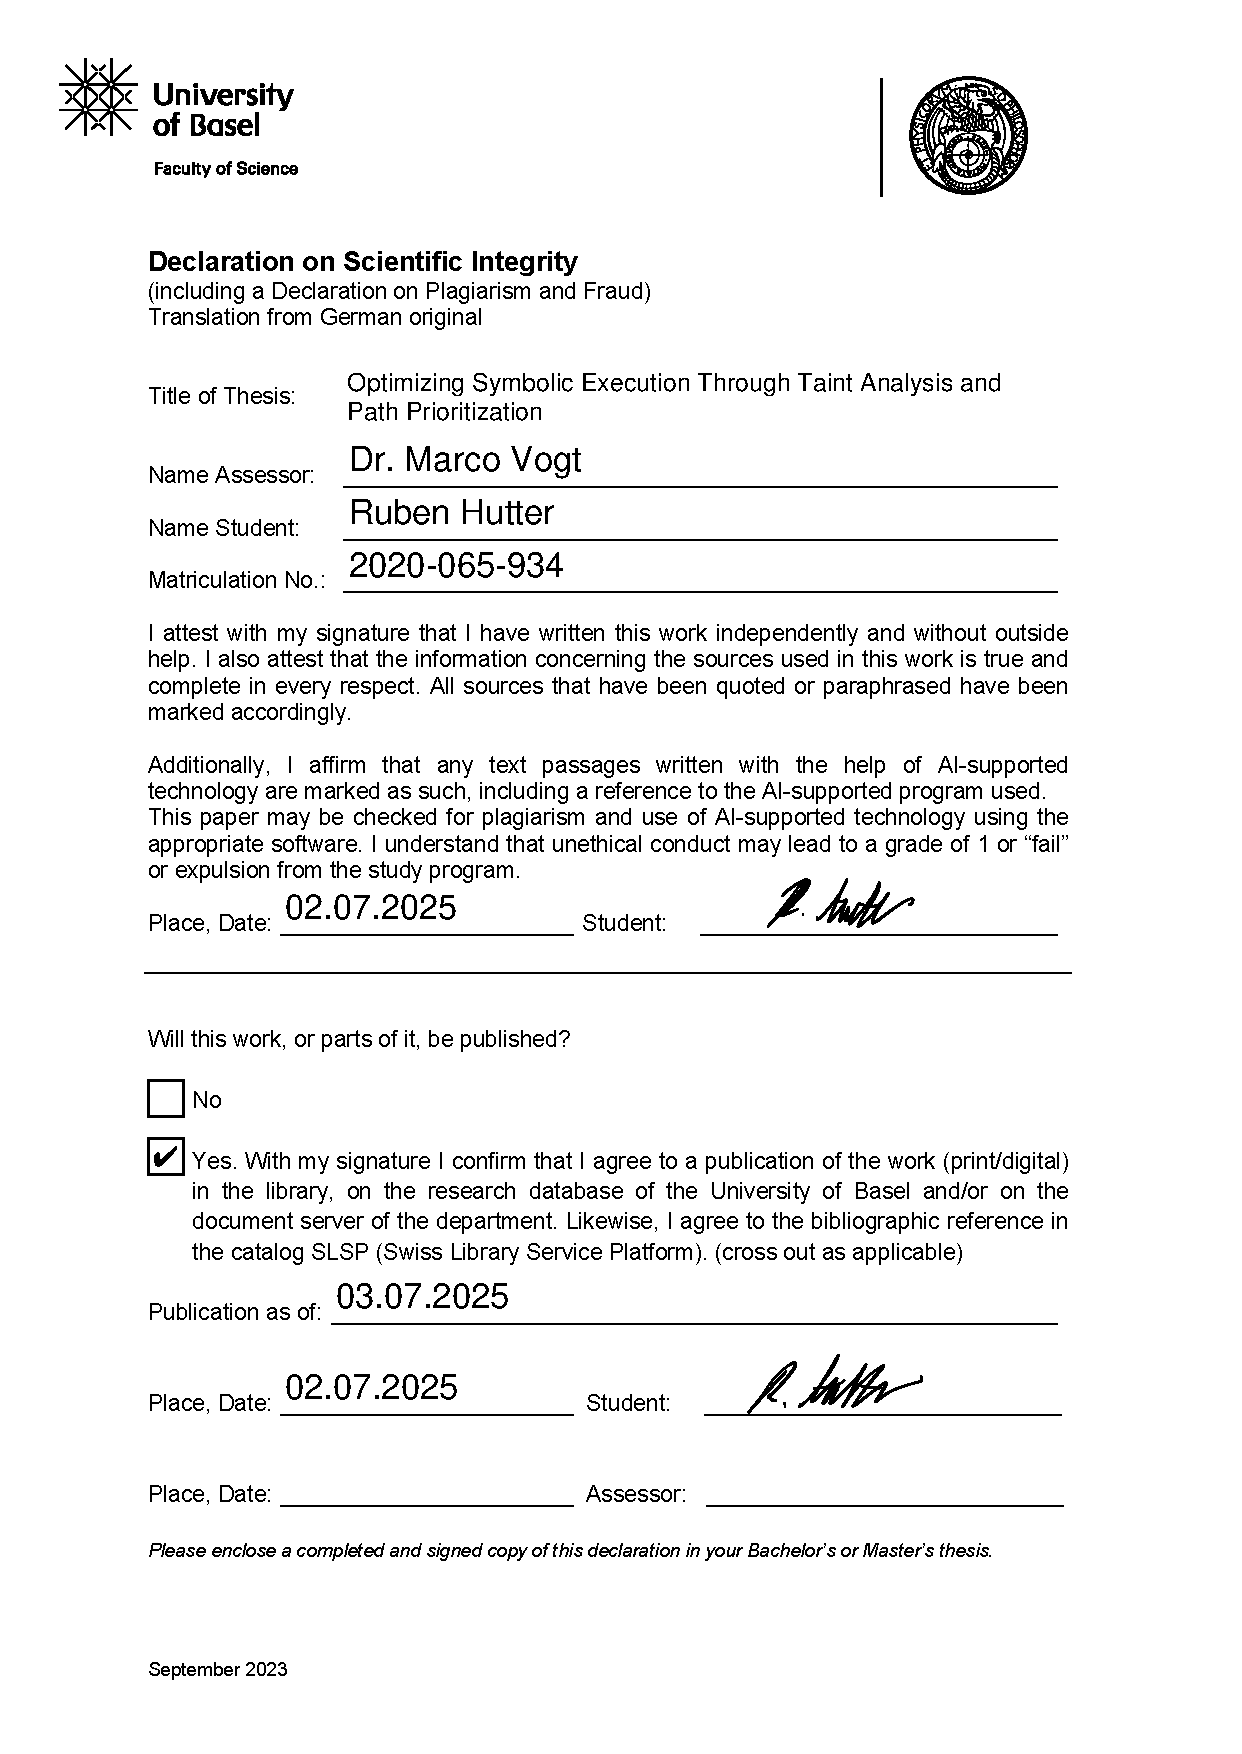
\includepdf{./Back/wissensch_Redlichkeit_E_09-2023.pdf}}
  {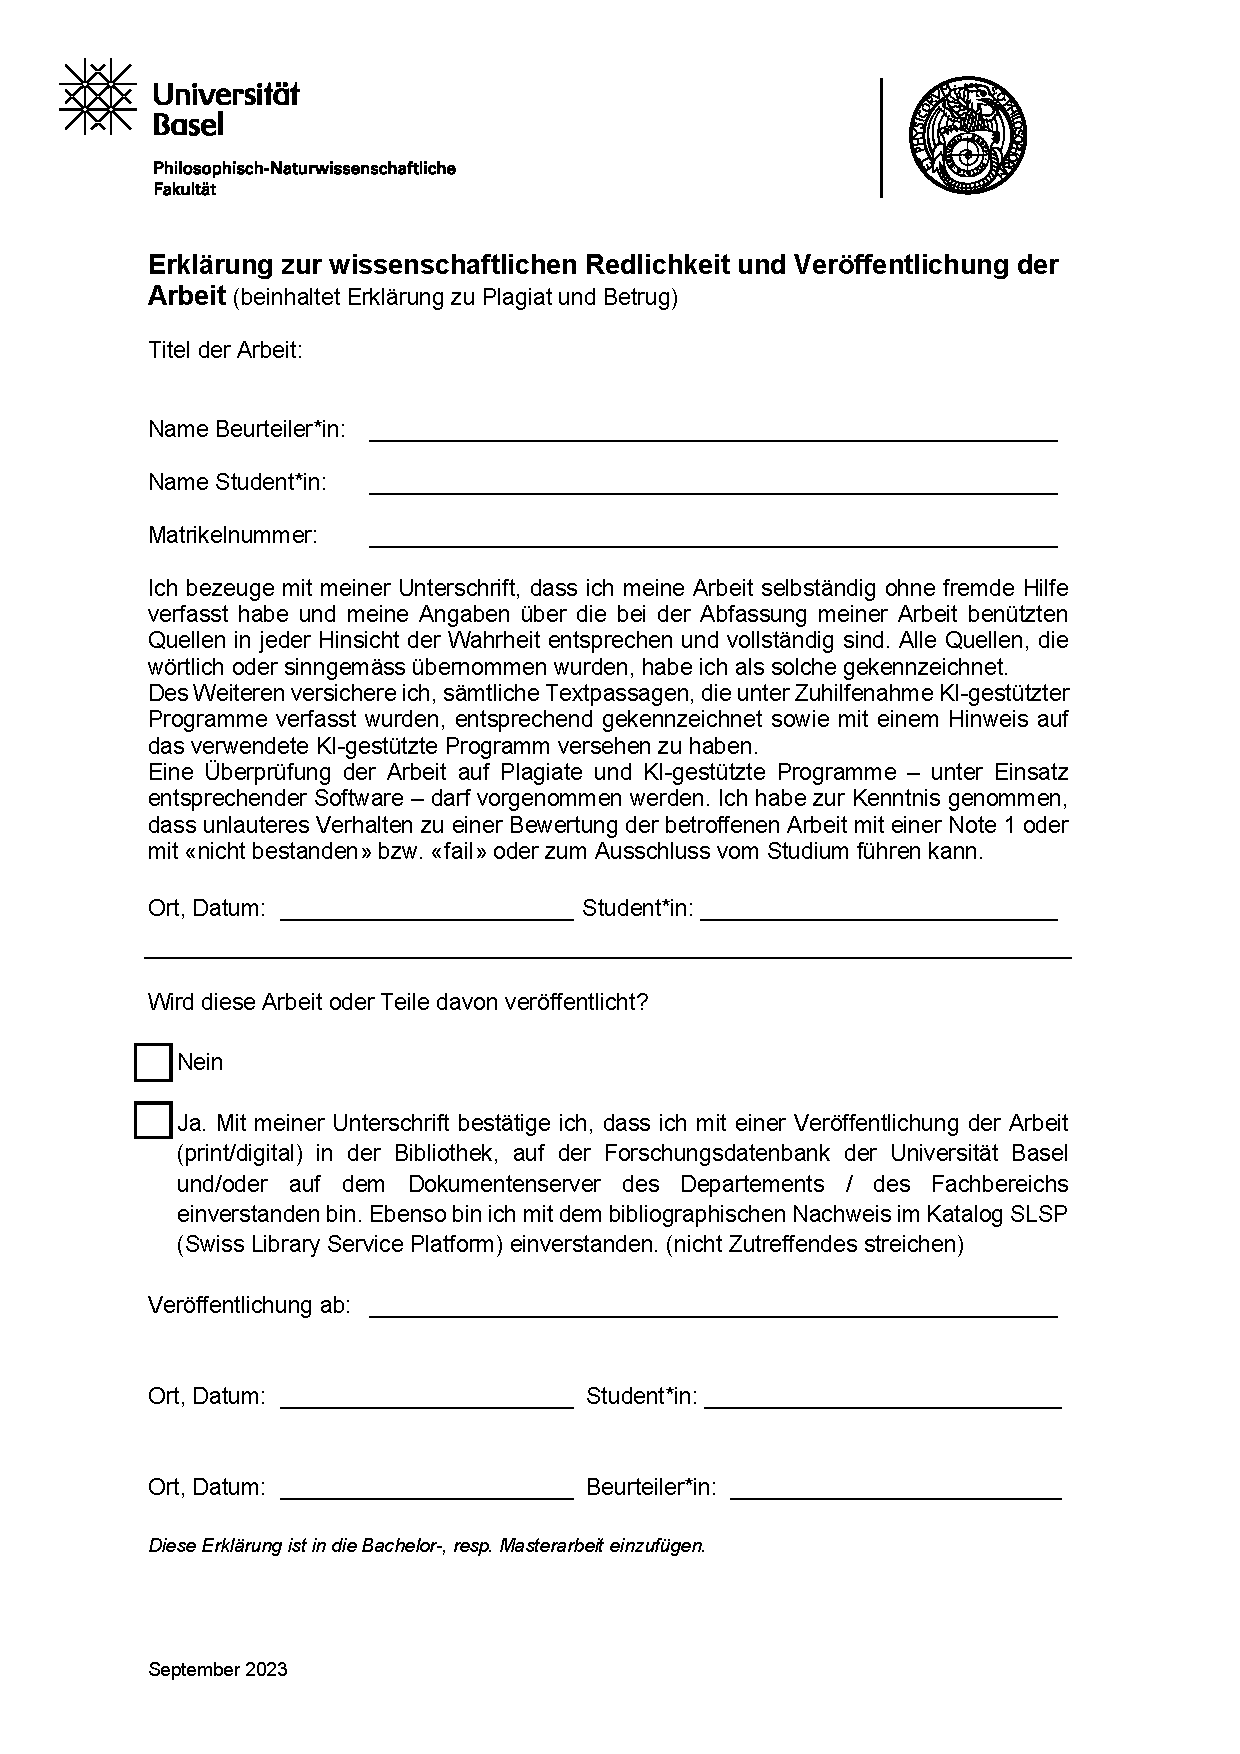
\includepdf{./Back/wissensch_Redlichkeit_D_09-2023.pdf}}
%% ----------------------------------------------------------------
\end{document}
%% ----------------------------------------------------------------
